\documentclass[12pt,a4paper]{article}

% ── Packages ──────────────────────────────────────────────────────
\usepackage{amsmath,amssymb,amsthm}
\usepackage{booktabs}
\usepackage{geometry}
\usepackage{hyperref}
\usepackage{microtype}
\usepackage{graphicx}
\usepackage{xcolor}
\usepackage{setspace}
\usepackage{parskip}

\geometry{margin=1in}
\onehalfspacing
\hypersetup{
  colorlinks=true,
  linkcolor=blue!60!black,
  citecolor=blue!60!black,
  urlcolor=blue!60!black
}

% ── Title ─────────────────────────────────────────────────────────
\title{Transient Geodesic Alignment in Life-Like Cellular Automata\\
on the \{7,3\} Heptagrid: Empirical Findings\\
and a Structural Mechanism}

\author{Clinton Foster\\
\small Independent Researcher\\
\small \href{https://github.com/TibbinQuickcoil/heptagrid-ca}{github.com/TibbinQuickcoil/heptagrid-ca}}

\date{}

% ── Document ──────────────────────────────────────────────────────
\begin{document}

\maketitle

% ── Abstract ──────────────────────────────────────────────────────
\begin{abstract}
We report an empirical investigation of two-state totalistic cellular automata on the $\{7,3\}$ heptagrid --- the regular tiling of the hyperbolic plane by heptagons meeting three to a vertex --- implemented in the Poincar\'{e} disk model with a 7-neighbor topology. While prior work on hyperbolic cellular automata has focused predominantly on questions of computational universality, the dynamical behavior of Life-like birth-survival rule families on this tiling remains largely uncharacterized. We introduce a geodesic alignment metric defined as the mean angular distance between alive-cell positions and the nearest of seven primary geodesic directions through the disk center, with a random baseline of $12.857°$ derived analytically. Surveying eight Life-like rule families across random initial conditions on grids of depth~4 (190~cells) and depth~5 (519~cells), we find that under rule B2/S23, all twenty tested random initial conditions at both grid sizes produce minimum alignment scores below the random baseline: mean minimum $7.998°$ (37.8\% below baseline) at depth~4, and $9.516°$ (26.0\% below baseline) at depth~5. The effect is transient, appearing during the early growth phase and relaxing toward baseline as grid occupancy increases. We derive a structural mechanism from two properties of the $\{7,3\}$ neighbor graph --- concentration of geodesic adjacency along geodesic directions (7.5--11.6$\times$ ratio at depth~4) and differential shared-neighbor density between on- and off-geodesic cell pairs --- both rule-independent properties of the tiling that intensify at larger scales. We also retract an initially observed period-4 oscillator under B34/S234, which does not persist at depth~5 and is a finite-grid artifact. The interactive computational explorer and all verification code are released as open-source artifacts.
\end{abstract}

% ── 1. Introduction ───────────────────────────────────────────────
\section{Introduction}

Conway's Game of Life \cite{Gardner1970} is among the most studied dynamical systems in mathematics. Half a century of investigation on the Euclidean square lattice has yielded a vast catalog of behaviors: still lifes, oscillators, gliders, glider guns, and computational structures sufficient to construct universal Turing machines. The square grid has become so naturalized as a substrate that the question of \emph{which substrate} is rarely asked. Yet the choice of underlying tiling is not neutral: it determines neighborhood structure, growth rates, and the geometric constraints under which patterns evolve.

The hyperbolic plane offers a substantially different substrate. Where the Euclidean plane admits regular tilings by squares, triangles, and hexagons, the hyperbolic plane admits an infinite family of regular tilings $\{p,q\}$ for which the angular constraint $(p-2)(q-2)>4$ is satisfied. Among these, the $\{7,3\}$ tiling --- heptagons meeting three to a vertex, the dual of the $\{3,7\}$ triangular tiling --- is the simplest hyperbolic regular tiling that produces a 7-neighbor cell structure. As the dual of the triangular tiling, the $\{7,3\}$ heptagrid has the lowest vertex valency among hyperbolic regular tilings, making it the sparsest such structure in terms of inter-cell connectivity per cell --- a property directly relevant to the sparse-field dynamics we analyze. Each cell touches exactly seven neighbors, the number of cells at graph distance $n$ from any given cell grows exponentially rather than quadratically, and straight lines through the plane are realized as arcs of circles orthogonal to the disk boundary in the Poincar\'{e} model.

A small but significant body of work has explored cellular automata on hyperbolic tilings \cite{Margenstern2000,Margenstern2007}. This literature has focused almost exclusively on computational universality: whether the substrate admits cellular automata capable of simulating arbitrary Turing machines. These are top-down constructions in which transition rules are explicitly engineered, often using geodesic paths as designed communication channels.

The complementary question --- what spontaneously emergent dynamical behavior arises when simple Life-like birth-survival rules are run on the $\{7,3\}$ tiling --- has received little attention. The closest prior exploration of which we are aware is an informal investigation by Mishin \cite{Mishin2011}, conducted on the $\{5,4\}$ pentagrid without quantitative analysis.

We are interested in a specific question: does the curvature of the underlying space leave detectable fingerprints on the dynamics of Life-like rules, even when those rules are themselves geometrically blind? A cellular automaton rule contains no representation of geodesics, distance, or curvature. It counts neighbors and applies a transition function. If the geometry of the substrate nevertheless biases the resulting dynamics, that bias must enter through the topology of the neighborhood graph alone.

We approach this question empirically, then mechanistically, and then critically --- explicitly testing initial findings across grid sizes and retracting one that does not survive. The remainder of the paper is organized as follows. Section~\ref{sec:methods} describes the tiling construction, CA implementation, and geodesic alignment metric. Section~\ref{sec:survey} presents the initial depth-4 survey. Section~\ref{sec:mechanism} derives the structural mechanism. Section~\ref{sec:validation} presents depth-5 validation and the retraction. Section~\ref{sec:limitations} addresses limitations and future work.

% ── 2. Methods ────────────────────────────────────────────────────
\section{Methods}
\label{sec:methods}

\subsection{Tiling Construction}

We work in the Poincar\'{e} disk model, in which the hyperbolic plane is represented as the open unit disk $\mathbb{D}=\{z\in\mathbb{C}:|z|<1\}$ with metric $ds=2|dz|/(1-|z|^2)$. Hyperbolic geodesics are diameters of the disk and arcs of circles meeting the boundary orthogonally.

The $\{7,3\}$ tiling is generated by reflecting a central heptagon across its sides recursively. Two geometric constants are derived from the Schl\"{a}fli symbol $\{7,3\}$ using standard formulas for regular hyperbolic polygons \cite{Coxeter1954}:
\begin{align}
R_c &= \cosh^{-1}\!\left(\frac{\cos(\pi/3)}{\sin(\pi/7)}\right) \approx 0.545
  \qquad\text{(circumradius: center to vertex)}\label{eq:Rc}\\[4pt]
r   &= \cosh^{-1}\!\left(\frac{\cos(\pi/7)}{\sin(\pi/3)}\right) \approx 0.283
  \qquad\text{(inradius: center to edge midpoint)}\label{eq:r}
\end{align}

The Euclidean displacement parameter for center-to-center moves in the Poincar\'{e} disk is $\rho_{cc}=\tanh(R_c)$, used to place adjacent cell centers via M\"{o}bius transforms of the form $T_{z_0,\theta}(z)=(z+z_0)/(1+\bar{z}_0 z)$.

For rendering cell boundaries, vertices are placed at Euclidean displacement $\rho_v=\tanh(D/2)$ where
\[
  D = \cosh^{-1}\!\bigl(\cosh(R_c)\cosh(r)\bigr) \approx 0.621.
\]
The geometric interpretation of $D$ as a standard $\{7,3\}$ polygon quantity requires independent verification and is not claimed here; $\rho_v$ is used for visualization only and does not enter into the CA logic or alignment metric.

\paragraph{Correction note.} An earlier draft of this paper mislabeled $R_c$ as ``apothem'' and $r$ as ``half-edge,'' reversing the standard definitions. This was a textual error identified in peer review (see Acknowledgments). The implementation correctly uses $\rho_{cc}=\tanh(R_c)$ for cell-center placement, verified to produce a valid $\{7,3\}$ neighbor graph by confirming each interior cell resolves exactly 7 neighbors.

Cell positions are enumerated by breadth-first search (BFS) beginning at the origin. From each cell, seven neighbors are generated at angles $\theta_j=\phi+2\pi j/7$ for $j=0,\ldots,6$, where $\phi$ is the local orientation inherited from the BFS. Cells within radius $0.971$ of the origin are retained for depth~4 ($N=190$ cells) and $0.989$ for depth~5 ($N=519$ cells). All runs use fixed initial orientation $\phi=0$ at the origin, ensuring deterministic BFS order.

The center cell lies at the origin with seven immediate neighbors (depth~1) at angles $2\pi j/7$ for $j=0,\ldots,6$ --- exactly along the seven primary geodesic directions. This is consequential for metric interpretation (\S\ref{sec:metric}).

\subsection{Cellular Automaton}

We implement two-state totalistic Life-like CA in the B/S family. The state of cell $i$ at time $t+1$ is:
\[
  s_i^{t+1} =
  \begin{cases}
    1 & \text{if } s_i^t=0 \text{ and } a_i\in B \\
    1 & \text{if } s_i^t=1 \text{ and } a_i\in S \\
    0 & \text{otherwise}
  \end{cases}
\]
where $a_i=\sum_{j\in\mathcal{N}(i)}s_j^t$ and $B,S\subseteq\{0,\ldots,7\}$. Eight rule families were surveyed: B3/S34, B2/S34, B23/S34, B3/S23, B2/S23, B34/S234, B2/S345, and B1/S12.

\subsection{Geodesic Alignment Metric}
\label{sec:metric}

For a cell at Poincar\'{e} disk coordinates $(c_r,c_i)$, define angular position $\theta=\arctan_2(c_i,c_r)$. The angular distance to the nearest of the seven primary geodesic directions $\{2\pi j/7\}$ is:
\[
  \delta(\theta) = \min\!\left(t,\;\frac{2\pi}{7}-t\right),
  \qquad t = \theta\bmod\frac{2\pi}{7}.
\]
The geodesic alignment score for a given generation is:
\[
  A = \frac{1}{|F|}\sum_{c\in F}\delta(\theta_c)\cdot\frac{180}{\pi}
\]
where $F$ is the set of alive cells with $c_r^2+c_i^2>0.002$. Lower $A$ indicates greater concentration near geodesic directions.

\paragraph{Random baseline.} For angular position drawn uniformly from $[0,2\pi)$:
\[
  \mathbb{E}[\delta] = \frac{\pi}{14} \approx 0.2244\;\text{rad} \approx 12.857°.
\]
This baseline assumes uniformly random angles. Since initial conditions are random by cell (not by angle), a slight geometric bias may exist at $t=0$ due to non-uniform angular density of cells at different depths in the Poincar\'{e} disk compression. We do not expect this to materially affect results as the effect is symmetric across geodesic sectors, but note it for completeness.

\paragraph{Geodesic threshold.} We use a secondary threshold of $7.071°\approx12.857°\times 0.55$ as an operational marker for strong geodesic bias. This threshold was chosen to clearly separate the null distribution from cases of marked concentration and does not derive from first principles.

\paragraph{Depth-1 caveat.} Depth-1 cells are placed exactly at geodesic directions by the BFS construction, contributing $\delta=0$ regardless of dynamics. Depth-stratified analysis accompanies aggregate scores throughout.

% ── 3. Initial Survey ─────────────────────────────────────────────
\section{Initial Survey --- Depth-4 Grid}
\label{sec:survey}

\subsection{Rule Survey Overview}

Table~\ref{tab:survey} summarizes the behavior of each rule family under random initial conditions (density 0.28, 20 seeds, 100 generations) on the 190-cell depth-4 grid.

\begin{table}[h]
\centering
\caption{Rule survey results, depth-4 grid (190 cells), 20 random seeds (density 0.28), 100 generations.}
\label{tab:survey}
\begin{tabular}{llccl}
\toprule
Rule & Alive@100 (mean) & Mean min align & Below baseline & Behavior \\
\midrule
B3/S34   & 0    & ---    & ---   & extinction \\
B2/S34   & 2    & 8.39°  & 20/20 & near-extinction \\
B23/S34  & $\sim$44 & 11.38° & partial & diffuse oscillation \\
B3/S23   & 3    & 8.57°$^{\dagger}$ & --- & depth-0/1 cluster \\
\textbf{B2/S23} & $\sim$38 & \textbf{7.998°} & \textbf{20/20} & \textbf{transient geodesic bias} \\
B34/S234 & 36--40 & 11.44° & partial & oscillatory (retracted --- see \S\ref{sec:retraction}) \\
B2/S345  & 0    & ---    & ---   & extinction \\
B1/S12   & $\sim$73 & 12.27° & partial & dense diffuse \\
\bottomrule
\end{tabular}
\vspace{4pt}
\begin{flushleft}
\small $^{\dagger}$B3/S23 dominated by depth-0/1 cluster; see \S\ref{sec:metric}.
\end{flushleft}
\end{table}

\subsection{B2/S23: Transient Geodesic Alignment}

Under B2/S23, all twenty random initial conditions produce minimum alignment below 12.857°. Full distribution of minima:

\begin{center}
4.17°, 5.71°, 7.34°, 7.35°, 7.39°, 7.48°, 7.68°, 7.75°, 7.89°, 8.01°,\\
8.34°, 8.35°, 8.38°, 8.40°, 8.49°, 8.68°, 9.00°, 9.28°, 9.60°, 9.61°
\end{center}

\begin{itemize}
  \item Mean minimum: $\mathbf{7.998°}$ (37.8\% below baseline)
  \item Below 7.071° threshold: 2/20
  \item Below baseline: 20/20
\end{itemize}

The minimum occurs at variable generations (9--71) during the intermediate-density growth phase, before relaxing toward baseline as grid occupancy increases. Figure~\ref{fig:trajectories} shows alignment trajectories for five representative seeds alongside the B1/S12 null result.

\paragraph{Depth-stratified analysis.} At the global minimum (seed~7, generation~34, 12 alive cells):

\begin{table}[h]
\centering
\caption{Depth-stratified alignment at minimum (seed 7, generation 34).}
\label{tab:depth}
\begin{tabular}{ccrl}
\toprule
Depth & Alive cells & Alignment & Note \\
\midrule
1 & 6 & 0.00° & geometric artifact \\
2 & 2 & 7.85° & sub-baseline, genuine signal \\
3 & 3 & 10.56° & near-baseline \\
4 & 1 & 2.63° & sub-baseline, small sample \\
\bottomrule
\end{tabular}
\end{table}

Excluding depth-1 cells: 6 remaining cells at depths 2--4 show mean alignment $7.43°$, below baseline.

\subsection{Null Results}

Five of eight rules produce no evidence of geometric organizing influence, confirming that geodesic bias is not a generic property of Life-like rules on the $\{7,3\}$ tiling but a feature of specific dynamical regimes.

\begin{figure}[h]
\centering
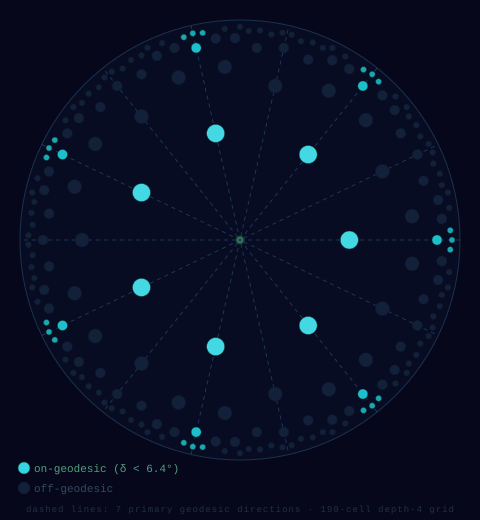
\includegraphics[width=0.75\textwidth]{figures/fig1_geodesic.pdf}
\caption{Geodesic classification of cells in the depth-4 $\{7,3\}$ Poincar\'{e} disk. Cyan cells are on-geodesic ($\delta<6.4°$); gray cells are off-geodesic. Dashed lines show the seven primary geodesic directions. On-geodesic cells form elongated radial chains; off-geodesic cells form dense interstitial regions.}
\label{fig:geodesic}
\end{figure}

\begin{figure}[h]
\centering
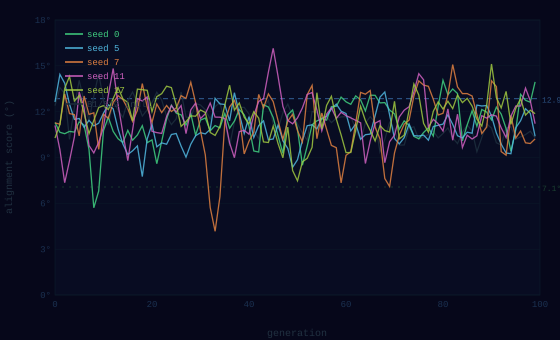
\includegraphics[width=0.85\textwidth]{figures/fig2_trajectory.pdf}
\caption{Geodesic alignment score over 100 generations under B2/S23 for five representative seeds (colored lines) and B1/S12 null result (dark line). Dashed line at $12.857°$ is the random baseline; dotted line at $7.071°$ is the strong bias threshold. All B2/S23 seeds descend below baseline during the growth phase before relaxing.}
\label{fig:trajectories}
\end{figure}

% ── 4. Mechanism ──────────────────────────────────────────────────
\section{Mechanism: Structural Origin of Geodesic Bias}
\label{sec:mechanism}

\subsection{Approach}

The transient alignment in B2/S23 admits two explanations: a statistical artifact of finite-grid effects or sampling noise, or a structural property of the $\{7,3\}$ neighbor graph that systematically favors geodesic propagation for certain rule families. We test the second hypothesis directly from the neighbor graph, independent of any rule or dynamics.

\subsection{Geodesic Classification}

We label each cell at depth $d\geq 1$ as \emph{on-geodesic} if $\delta(\theta_c)<\pi/28\approx6.43°$ --- within the inner half of the angular distance to the nearest geodesic --- and \emph{off-geodesic} otherwise.

\subsection{Geodesic Neighborhood Concentration}

For each cell, we count the number of its seven neighbors that are themselves on-geodesic.

\begin{table}[h]
\centering
\caption{Mean on-geodesic neighbors per cell, depth-4 grid.}
\label{tab:concentration}
\begin{tabular}{ccrrc}
\toprule
Depth & Class & $n$ & Mean on-geodesic neighbors & Ratio \\
\midrule
3 & on-geodesic  & 21 & 3.000 & \multirow{2}{*}{$7.5\times$} \\
3 & off-geodesic & 35 & 0.400 & \\[4pt]
4 & on-geodesic  & 21 & 1.667 & \multirow{2}{*}{$10.0\times$} \\
4 & off-geodesic & 84 & 0.167 & \\
\bottomrule
\end{tabular}
\end{table}

At depth~3, on-geodesic cells have $7.5\times$ more on-geodesic neighbors than off-geodesic cells of the same depth. At depth~4 the ratio is $10.0\times$. This is a purely structural property of the $\{7,3\}$ tiling derived from the neighbor graph, independent of any rule or initial condition.

\subsection{Shared Neighbor Density}

\begin{table}[h]
\centering
\caption{Mean shared neighbors among adjacent cell pairs, depth-4 grid.}
\label{tab:shared}
\begin{tabular}{lcc}
\toprule
Pair type & $n$ pairs & Mean shared neighbors \\
\midrule
Both on-geodesic  & 35  & 0.800 \\
Both off-geodesic & 161 & 1.043 \\
\bottomrule
\end{tabular}
\end{table}

Off-geodesic adjacent pairs share 30\% more neighbors than on-geodesic pairs (1.043 vs.\ 0.800). The on-geodesic chain topology is sparsely cross-connected; off-geodesic regions are densely cross-connected.

\subsection{The Two-Component Mechanism}

\paragraph{Component~1 --- Directed alive signal.}
During sparse growth, an on-geodesic cell has $7.5$--$10\times$ more geodesic-adjacent neighbors than an off-geodesic cell at the same depth. If any chain cell becomes alive, its on-geodesic neighbors receive a concentrated alive-cell signal in the chain direction, biasing the probability of satisfying B2 (exactly 2 alive neighbors) along geodesics.

\paragraph{Component~2 --- Differential birth probability by neighbor-count rule.}
The dense cross-connectivity of off-geodesic regions pushes alive-neighbor counts above the B2 threshold, suppressing B2 birth. Crucially, this mechanism \emph{inverts} for higher birth-count rules: for B3 or B4 rules, dense cross-connectivity facilitates rather than suppresses birth by making it easier to accumulate 3 or more simultaneous alive neighbors. This predicts a dichotomy: B2-family rules exhibit geodesic bias through birth-suppression off-geodesic, while B3-family rules show reduced or absent bias --- consistent with our null results for all B3-based rules in the survey.

\paragraph{Transience.}
The mechanism is density-dependent. As the alive-cell density increases, the structural advantage of on-geodesic cells diminishes relative to total alive-neighbor counts, and the alignment signal relaxes toward baseline.

\subsection{Status of the Argument}

The structural properties in Tables~\ref{tab:concentration} and~\ref{tab:shared} are computed exactly from the $\{7,3\}$ neighbor graph and are rule-independent. The prediction that B2/S23 exhibits transient geodesic bias follows under a qualitative argument about sparse-field birth probabilities. A complete formal derivation --- computing birth probabilities explicitly as a function of density and cell classification --- is the principal direction for future theoretical work. The structural concentration ratios (7.5--10$\times$) are too large to be explained by finite-grid noise, ruling out the sampling-artifact hypothesis.

% ── 5. Depth-5 Validation ─────────────────────────────────────────
\section{Depth-5 Validation}
\label{sec:validation}

\subsection{B2/S23 at Depth~5}

Twenty seeds were tested at 150 generations on the depth-5 grid ($N=519$).

\begin{table}[h]
\centering
\caption{B2/S23 geodesic alignment by grid depth.}
\label{tab:scales}
\begin{tabular}{lcccccc}
\toprule
Grid & $N$ & Mean min & Reduction & Below baseline & Below $7.071°$ \\
\midrule
Depth 4 & 190 & 7.998° & 37.8\% & 20/20 & 2/20 \\
Depth 5 & 519 & 9.516° & 26.0\% & 20/20 & 0/20 \\
\bottomrule
\end{tabular}
\end{table}

The directional finding is confirmed: 20/20 seeds below baseline at both grid sizes. The magnitude weakens from 37.8\% to 26.0\%, and no depth-5 seed breaches the strong threshold.

Individual depth-5 minima: 8.80°, 8.86°, 8.99°, 9.12°, 9.12°, 9.19°, 9.26°, 9.28°, 9.34°, 9.44°, 9.47°, 9.53°, 9.58°, 9.72°, 9.82°, 9.98°, 10.02°, 10.10°, 10.34°, 10.38°.

\subsection{Retraction: B34/S234 Period-4 Oscillator}
\label{sec:retraction}

At depth~4, rule B34/S234 produced a repeating alive-count cycle $(39,37,40,36)$ by approximately generation~40, persisting through generation~100 across all tested seeds. At depth~5, no such clean periodicity is observed within 120 generations. The depth-4 cycle is a finite-grid artifact specific to the 190-cell grid.

We retract this finding. The period-4 oscillator was real within the 190-cell grid; it is not a property of the rule on the infinite $\{7,3\}$ tiling. This retraction is reported as an example of standard scientific practice.

\subsection{Structural Mechanism at Depth~5}

\begin{table}[h]
\centering
\caption{Geodesic neighborhood concentration, depth-5 grid.}
\label{tab:depth5struct}
\begin{tabular}{cccc}
\toprule
Depth & On-geo mean & Off-geo mean & Ratio \\
\midrule
3 & 3.667 & 0.400 & $9.17\times$ \\
4 & 5.800 & 0.500 & $11.60\times$ \\
5 & 1.400 & 0.000 & not computed (see text) \\
\bottomrule
\end{tabular}
\end{table}

At depth~5, off-geodesic cells show zero on-geodesic neighbors. This is a boundary artifact: depth-5 cells have neighbors at depth~6, which fall outside the radius cutoff. The depth-5 ratio is therefore a lower bound on the true structural concentration rather than a property of the infinite tiling. Division by zero is not performed. The ratios at depths~3 and~4, where both cell classes have fully resolved neighbors, show genuine intensification ($7.5\times$ to $9.17\times$ at depth~3; $10.0\times$ to $11.6\times$ at depth~4).

\subsection{Reconciling Stronger Mechanism with Weaker Signal}

The structural concentration strengthens at depth~5 while the aggregate alignment signal weakens. This is explained by population averaging: at depth~5 the total alive-cell population is larger, and the geodesic chains form a smaller fraction of the total. The aggregate metric averages over all alive cells including the large off-geodesic population contributing near-baseline values.

The invariant result across both scales is the directional one: 20/20 seeds below baseline at both depths. This is the most defensible form of the primary finding.

% ── 6. Limitations ────────────────────────────────────────────────
\section{Limitations and Future Work}
\label{sec:limitations}

\paragraph{Formal derivation.}
The mechanism in \S\ref{sec:mechanism} is structurally grounded but not formally proven. A complete derivation would compute birth probabilities as a function of density and cell classification, yielding a quantitative prediction testable against the alignment trajectory.

\paragraph{Euclidean control.}
Running the same rule families on a square or hexagonal grid with an analogous angular metric is the most important missing validation. This would test whether the effect is specific to hyperbolic curvature or could arise from any regular tiling with preferred directions.

\paragraph{Larger grids.}
Depth~6 yields approximately $N\approx 1900$ cells. The population-averaging hypothesis (\S\ref{sec:validation}) could be tested directly via depth-stratified alignment at depth~5, which would then be estimable from a sufficient cell sample. The depth-5 structural boundary artifact would also be resolved.

\paragraph{Rule space coverage.}
The full two-state totalistic rule space on a 7-neighbor grid contains $2^8\times 2^8=65{,}536$ rules. Systematic exploration of B2-family rules is a natural extension.

\paragraph{Geometric constant verification.}
The vertex placement parameter $\rho_v=\tanh(D/2)$ is used for rendering only. Its geometric interpretation as a standard $\{7,3\}$ polygon quantity requires independent derivation.

% ── 7. Conclusion ─────────────────────────────────────────────────
\section{Conclusion}

We have presented a quantitative empirical study of Life-like cellular automata on the $\{7,3\}$ heptagrid, tested at two grid scales, with a structural mechanism derived from the neighbor graph and an explicit retraction of one initial finding that did not survive scale testing.

The principal finding is that rule B2/S23 consistently produces transient sub-baseline geodesic alignment during early growth from random initial conditions: 20/20 seeds below the $12.857°$ random baseline at both depth~4 and depth~5, with mean minimum reductions of 37.8\% and 26.0\% respectively. The directional consistency across all forty tested conditions is the most defensible form of this result.

The structural mechanism --- concentration of geodesic adjacency ($7.5$--$11.6\times$ ratio at depth~4, with genuine intensification at depth~5) and differential shared-neighbor density --- is derived from properties of the $\{7,3\}$ neighbor graph independent of any rule or dynamics. The observation that the structural anisotropy strengthens at scale while the aggregate alignment signal weakens is explained as population averaging, constituting a testable prediction for future depth-stratified analysis at larger grids.

The B34/S234 period-4 oscillator does not persist at depth~5 and is retracted.

\medskip
\noindent Cellular automaton rules are geometrically blind. The $\{7,3\}$ tiling is not.

% ── Acknowledgments ───────────────────────────────────────────────
\section*{Acknowledgments}

The interactive computational explorer and Python verification scripts were developed with AI-assisted coding tools (Anthropic Claude). Empirical observations, methodological design, analytical framing, multi-scale validation, and the decision to retract the B34/S234 finding were developed through human-AI collaboration. All results were independently verified by Python reimplementation. Peer review commentary from Gemini~2.5 contributed the suggestion to note the $\{7,3\}/\{3,7\}$ duality and to sharpen the B3 mechanism dichotomy. Kimi identified the mislabeling of geometric constants in \S\ref{sec:methods}. Grok identified the numerical error in $R_c$ and validated the analytical baseline. DeepSeek identified the table-citation inconsistency and the inline citation formatting issue.

\section*{Code and Data Availability}

The interactive $\{7,3\}$ cellular automaton explorer with integrated geodesic alignment analysis, Python survey and mechanism scripts, raw data, and SVG figures are available at:
\begin{center}
\url{https://github.com/TibbinQuickcoil/heptagrid-ca}
\end{center}

% ── References ────────────────────────────────────────────────────
\begin{thebibliography}{9}

\bibitem{Gardner1970}
Gardner, M. (1970).
Mathematical games: The fantastic combinations of John Conway's new solitaire game ``life.''
\textit{Scientific American}, 223(4), 120--123.

\bibitem{Coxeter1954}
Coxeter, H.~S.~M. (1954).
Regular honeycombs in hyperbolic space.
\textit{Proceedings of the International Congress of Mathematicians, Amsterdam}, III, 155--169.

\bibitem{Margenstern2000}
Margenstern, M. (2000).
New tools for cellular automata in the hyperbolic plane.
\textit{Journal of Universal Computer Science}, 6(12), 1226--1252.

\bibitem{Margenstern2007}
Margenstern, M. (2007).
\textit{Cellular Automata in Hyperbolic Spaces, Volume~1: Theory}.
Old City Publishing.

\bibitem{MargensternMorita2001}
Margenstern, M., \& Morita, K. (2001).
NP problems are tractable in the space of cellular automata in the hyperbolic plane.
\textit{Theoretical Computer Science}, 259, 99--128.

\bibitem{Mishin2011}
Mishin, D. (2011).
Hyperbolic cellular automaton [informal exploration, $\{5,4\}$ pentagrid].
Retrieved from \url{http://dmishin.blogspot.com/2011/10/hyperbolic-cellular-automation.html}

\bibitem{Wolfram2002}
Wolfram, S. (2002).
\textit{A New Kind of Science}.
Wolfram Media.

\end{thebibliography}

\end{document}
